\documentclass[pdftex, a4paper, 11pt]{article}
\usepackage[italian]{babel}
\usepackage{fancyhdr,graphicx}
\usepackage[hmargin=2cm,vmargin=2cm,a4paper]{geometry}
\usepackage{hyperref}

\pagestyle{fancy}
\lhead{\scshape Curriculum Vitae}
\rhead{\itshape Enrico Carlesso}
\rfoot{\footnotesize pag. \thepage}
\cfoot{}
\lfoot{{\footnotesize Aggiornato al:} \today}
\renewcommand{\headrulewidth}{1pt}
\renewcommand{\footrulewidth}{1pt}

\begin{document}
\vspace*{.3cm}
\begin{center}
  \rule{.8\textwidth}{1pt}\\[10pt]
  \begin{minipage}{.55\textwidth}
    \LARGE\textbf{Enrico Carlesso}\\[13pt]
    \small Via Julia, 37\\
    36060 - Romano d'Ezzelino (VI)\\[6pt]
    \textbf{e-mail: enrico@ecarlesso.org}\\
    \small \url{http://www.ecarlesso.org}\\
    \small N. Tel: +39 348 858 77 86\\[6pt]
    \small Nazionalit\'a: Italiana\\
    %% \small Data di nascita: 03.12.1984\\
    \small Stato civile: celibe\\
  \end{minipage}
  \begin{minipage}{.2\textwidth}
    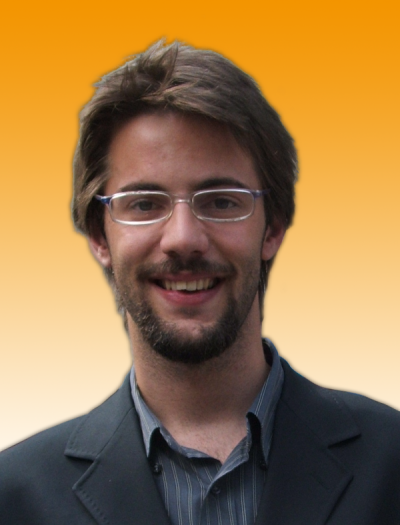
\includegraphics[width=\textwidth]{foto.png}
  \end{minipage}\\[5pt]
  \rule{.8\textwidth}{1pt}
\end{center}
\vspace*{1cm}

\section*{Posizione Attuale:}


Sviluppatore Freelance

Iscrizione al Registro Imprese con Partita IVA n. 03472460249 con qualifica di ``Consulente nel settore delle tecnologie dell'informatica''

% Stageaire presso la divisione R\&D di M31.

\section*{Istruzione}
\begin{itemize}
\item Laurea Specialistica in Ingegneria Informatica con votazione 101/110 (Universit\`a degli studi di Padova, 2011);
\item Laurea Triennale in Ingegneria Informatica con votazione 92/110 (Universit\`a degli
  studi di Padova, 2007);
\item Diploma di Ragioneria (I.T.C.G. L. Einaudi di Bassano del Grappa,
  2003).
\end{itemize}

\section*{Esperienze}
\begin{itemize}
\item Stage presso il reparto R\&D di M31;
\item Tesi presso M31 dal titolo ``Un sistema di monitoraggio e controllo remoto per dispositivi industriali'';
\item Realizzazione di progetti web per diversi clienti;
\item Fornitura di consulenze nell'ambito di creazione e manutenzione server;
\item Partecipazione al German Open 2007, con la squadra
  dell'universit\`a di Padova nella ``Humanoids Legue'';
\item Tesi presso il Laboratorio di Sistemi Autonomi ed
  Intelligenti dell'universit\`a di Padova dal titolo ``Algoritmi
  simultanei di localizzazione e mappatura basati sulla visione artificiale'';
\item Realizzazione di diverso software opensource,
  prevalentemente in Ruby e Python.
\end{itemize}

\section*{Compenze informatiche}
\begin{description}
\item[Web:] Ottima conoscenza dei framework RubyOnRails (Ruby), Django
  (Python) e CakePHP (php). Ottime capacit\'a in
  tutto ci\`o che riguarda il web. Ottima conoscenza
  di Javascript. Ottima conoscenza dei maggori Database: MySQL, PostgreSQL, MongoDB, Sqlite.
\item[S.O.:] GNU/Linux, Archlinux \& Slackware {\em in primis},
  ottima conoscenza
  in ogni campo, dall'installazione, alla configurazione, alla
  creazione di software di supporto. Ottima conoscenza del linguaggio
  {\em bash} ed ottime capacit\`a di realizzazione di script
  mirato. Ottima competenza in ambito server.
\item[Programmazione:] Ottima conoscenza di Ruby, Python e Javascript. Buone competenze in C e C++.
  Esperienze di programmazione con molti altri linguaggi;
\item[Altro:] \LaTeX, QT, vim, iptables, cups, samba, foss, gestione di reti.
\end{description}

\section*{Esperienze Lavorative}
\begin{itemize}
  \item Maggio 2008/Attualmente: Sviluppatore Freelance come libero professionista;
  \item Febbraio 2013/Febbraio 2015: Software Architect in Si14 SpA;
  \item Maggio 2011/Febbraio 2013: CTO per Doochoo Inc.;
  \item Aprile 2010/Marzo 2011: Ingegnere del software presso M31;
\item Gennaio/Maggio 2008: Assistenza hardware/software presso DV
  Service (Romano d'Ezzelino - VI);
\item Maggio/Ottobre 2007: Ricerca e sviluppo presso Zilio
  S.p.A. (Cassola - VI), con progettazione e vendita di un sistema di
  videosorveglianza basato su Linux e Videocamere ad alta definizione
  (5Mpx);
\item 1999/2004: Cameriere nei fine settimana presso Villa Razzolini
  Loredan (Asolo - TV);
\item Giugno/Ottobre 2002: Impiegato Tecnico presso ``IALC'' (Romano
  d'Ezzelino - VI).
\end{itemize}

%\section*{Progetti realizzati}
%\begin{itemize}
%\item pynokia: programma che permette l'invio di sms (e
  %altre interazioni) dal computer attraverso connessione
  %bluetooth/cavo a cellulari Nokia. {\em (Python)}\\
  %\url{http://github.com/carlesso/pynokia}
%\item videntify: programma per estrapolare informazioni da
  %file video. {\em (C)}\\
  %\url{http://www.ecarlesso.org/works/show/videntify}
%\item Freesky: scheda controllo motori da servomodellismo,
  %progettazione, assemblamento e firmware. {\em (Eagle, ARM-C)}\\
%%  \url{http://www.ecarlesso.org/index.php/freesky}
%\end{itemize}

%% \section*{Portfolio WEB}
%% \begin{description}
%% \item[cnssrl.it] Sito dell'azienda CNS srl, con catalogo prodotti
%%   e backend di amministrazione a misura del cliente. Basato su CakePHP
%%   e MooTools\\
%%   \url{http://www.cnssrl.it};
%% \item[ecarlesso.org] Sito personale, in continua crescita. Basato
%%   su CakePhP e MooTools\\
%%   \url{http://www.ecarlesso.org};
%% \end{description}

\section*{Interessi personali}
\begin{itemize}
\item Informatica generale;
\item Web e tecnologie ``cutting-edge'' come nuova esperienza per l'utente;
\item {\bf F}ree and {\bf O}pen {\bf S}ource {\bf S}oftware;
\item Matematica, con particolare attenzione all'algebra;
\item Interazione tra elettronica ed informatica;
\item Ottobre 2009 - Attualmente: GrappaLUG - Linux User Group di Bassano del Grappa;
\item Ottobre 2006 - Attualmente: Membro della Pro Loco di Romano d'Ezzelino.
\end{itemize}

\section*{Competenze Linguistiche}
\begin{description}
\item[Italiano:] Madrelingua;
\item[Inglese:] Ottimo livello di comprensione e scrittura;
\item[Tedesco:] Conoscenza didattica.
\end{description}

\section*{Nel web}
\begin{description}
\item[github.com] La maggior parte dei miei progetto risiede sulla mia pagina su github.com: \\ \mbox{\url{https://github.com/carlesso}};
\item[linkedin] La mia pagina su linkedin: \\ \url{http://www.linkedin.com/in/ecarlesso};
\item[stackoverflow.com] Il mio profilo su stackoverflow careers: \\ \url{http://careers.stackoverflow.com/ecarlesso}.
\end{description}

\vfill

%% Ai sensi della legge 675/96 (tutela della persona ed altri soggetti
%% rispetto al trattamento dei dati personali), autorizzo al trattamento
%% dei dati personali contenuti nel presente Curriculum Vitae per
%% permettere un adeguata valutazione della mia candidatura finalizzata all'assunzione.
Autorizzo il trattamento dei dati da me forniti ai sensi della legge
675/96 sulla privacy.

\vspace{1cm}

\footnotesize {Questo curriculum \`e disponibile come repository {\em git}. \`E possibile scaricare la versione aggiornata:}
\begin{verbatim}
    $ git clone git://github.com/carlesso/ecarlesso_cv.git
\end{verbatim}
\end{document}
